\documentclass{beamer}
\usetheme{Luebeck}
\usecolortheme{spruce}
\usepackage{animate}
\usepackage{tikz}

\usepackage{hyperref}
\usepackage{fancyhdr}

\usepackage{circuitikz}
\usetikzlibrary{arrows}
\usetikzlibrary{positioning}
\usetikzlibrary{overlay-beamer-styles}
\usetikzlibrary{circuits.ee.IEC, shapes.misc, shapes.geometric}

\title{Real-Time Keyword Recognition on STM32\\using TensorFlow Lite}
%\subtitle{Project Presentation}
\institute{ETH Zürich}
\author{Stefan Gloor}
\date{June 12, 2024}

\setbeamertemplate{navigation symbols}{}%remove navigation symbols
\setbeamertemplate{footline}[frame number]

\definecolor{mygreen}{RGB}{0,102,51}

\setbeamercolor*{structure}{bg=black,fg=mygreen!40}

\setbeamercolor*{palette primary}{use=structure,fg=black,bg=structure.fg}
\setbeamercolor*{palette secondary}{use=structure,fg=black,bg=structure.fg!75}
\setbeamercolor*{palette tertiary}{use=structure,fg=white,bg=structure.fg!50!black}
\setbeamercolor*{palette quaternary}{fg=black,bg=mygreen!30!white}

\setbeamercolor{section in toc}{fg=black,bg=mygreen}
\setbeamercolor{alerted text}{use=structure,fg=black}

\setbeamercolor{titlelike}{parent=palette primary,fg=black}
\setbeamercolor{frametitle}{bg=white,fg=black}

%\setbeamercolor*{titlelike}{parent=palette primary}
\setbeamertemplate{headline}{}
\usefonttheme[onlymath]{serif}

\begin{document}

\begin{frame}
	\titlepage
\end{frame}

\section*{Contents}
\begin{frame}{Contents}
\setbeamercolor{local structure}{fg=mygreen}
\setbeamercovered{transparent}
	\begin{itemize}
		\item<2->Project goals
		\item<3->Hardware
		\item<4->Dataset
		\item<5->Model and framework
		\item<6->Microcontroller Implementation
		\item<7->Performance evaluation
		\item<8->Limitations
		\item<9->Demo
	\end{itemize}
\end{frame}

\section{Project Goals}
\subsection{Motivation}
\begin{frame}{Motivation}
	\begin{minipage}{0.67\textwidth}
	\setbeamercolor{local structure}{fg=mygreen}
	\setbeamercovered{transparent}
	\begin{itemize}
		\item<2->Simple speech recognition
			\setbeamercolor{local structure}{fg=mygreen}
			\setbeamercovered{transparent}
			\begin{itemize}
				\item<3-> Wide range of applications
				\item<4-> Simple and cheap user interface
				\item<5-> Hands-free operation of devices
			\end{itemize}\vspace{5mm}

		\item<6-> Why on the edge?
			\setbeamercolor{local structure}{fg=mygreen}
			\setbeamercovered{transparent}
			\begin{itemize}
				\item<7-> Very cheap
				\item<8-> Low latency
				\item<9-> Data privacy
			\end{itemize}
			\end{itemize}
	\end{minipage}
	\begin{minipage}{0.24\textwidth}
		
\includegraphics[width=0.9\textwidth]{figures/microphone.png}
	\end{minipage}
\end{frame}

\subsection{Goals}
\begin{frame}{Goals}
	\begin{minipage}{0.67\textwidth}
	\setbeamercolor{local structure}{fg=mygreen}
	\setbeamercovered{transparent}
	\begin{itemize}
		\setlength\itemsep{1em}
		\item<2->Achieve simple speech recognition completely ``on the edge'',
			detect keywords such ``left'' and ``right''.
		\item<3->Familiarize with available frameworks
		\item<4->Demo project as a base for future applications
	\end{itemize}
	\end{minipage}
	\begin{minipage}{0.24\textwidth}
		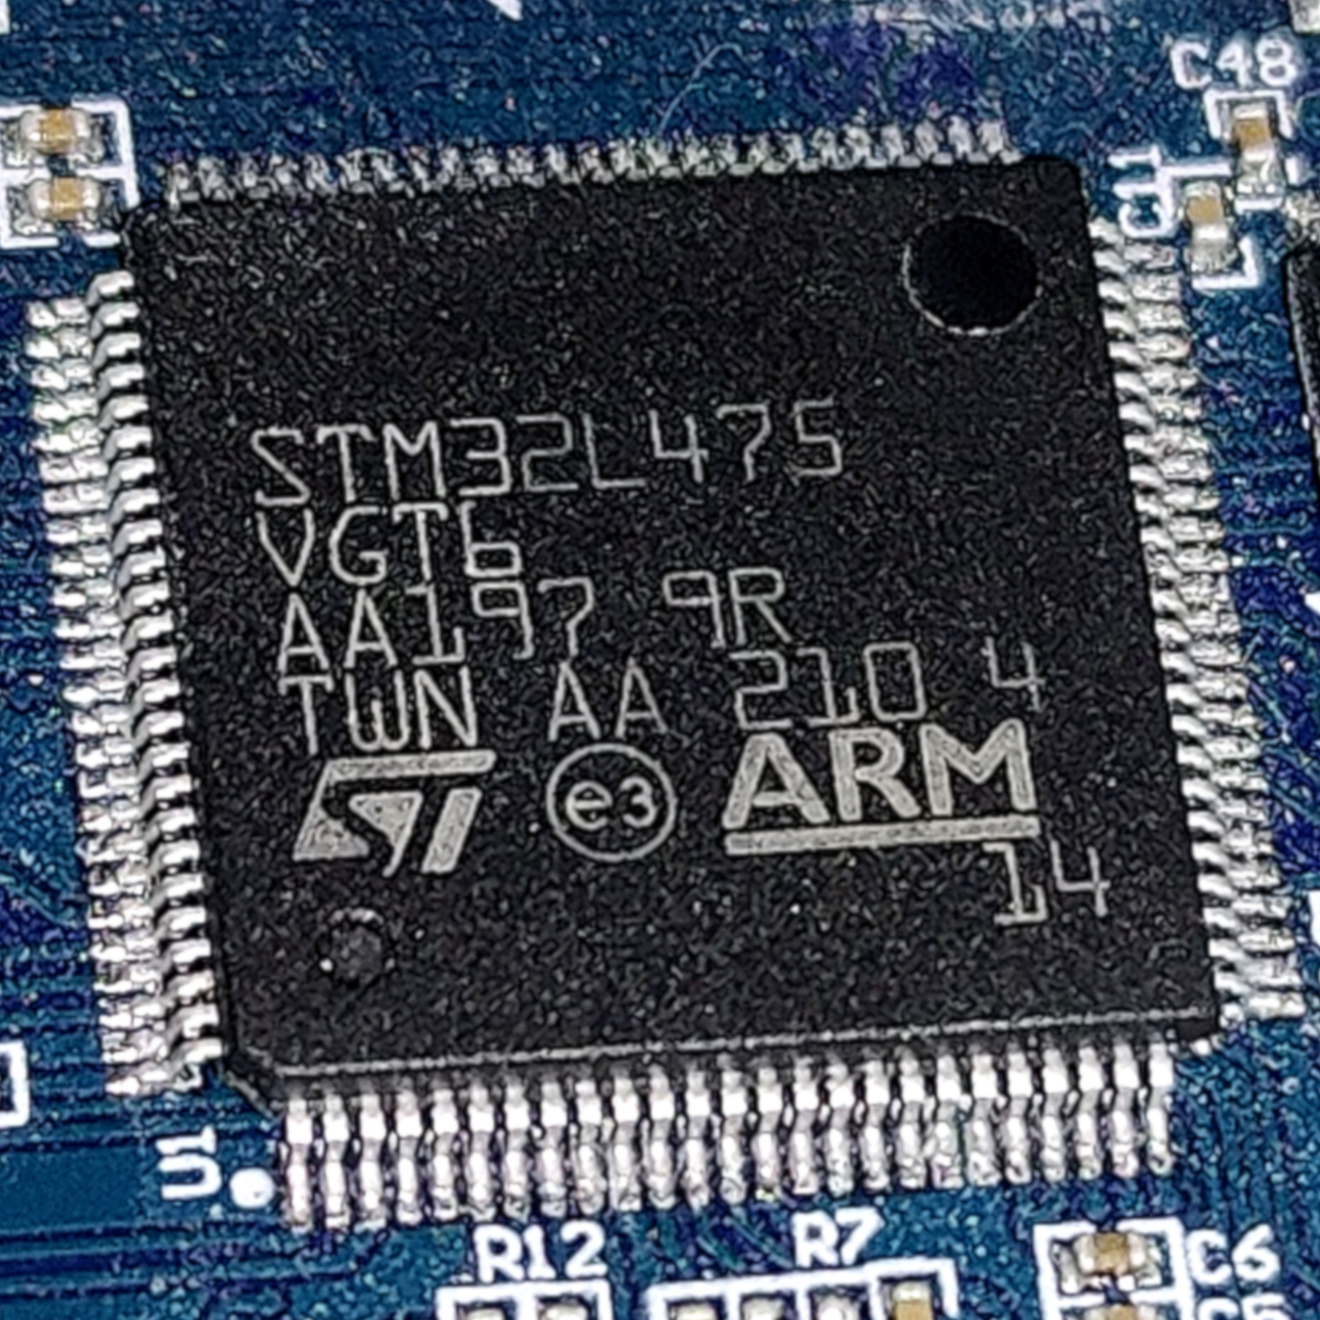
\includegraphics[width=0.9\textwidth]{figures/stm32l475.jpg}
	\end{minipage}
\end{frame}

\section{Hardware}
\begin{frame}{Hardware}
\begin{minipage}{0.5\textwidth}
	\setbeamercolor{local structure}{fg=mygreen}
	\setbeamercovered{transparent}
	\begin{itemize}
		\item<2->STM32L475VGT
			\setbeamercolor{local structure}{fg=mygreen}
			\setbeamercovered{transparent}
			\begin{itemize}
				\item<3-> General-purpose MCU
				\item<4-> Industry-proven
				\item<5-> Good availability
			\end{itemize}
		\item<6->Arm Cortex M4F @ 80 MHz
		\item<7->1 MB Flash
		\item<8->128 kB SRAM
	\end{itemize}
	\end{minipage}
	\begin{minipage}{0.48\textwidth}
		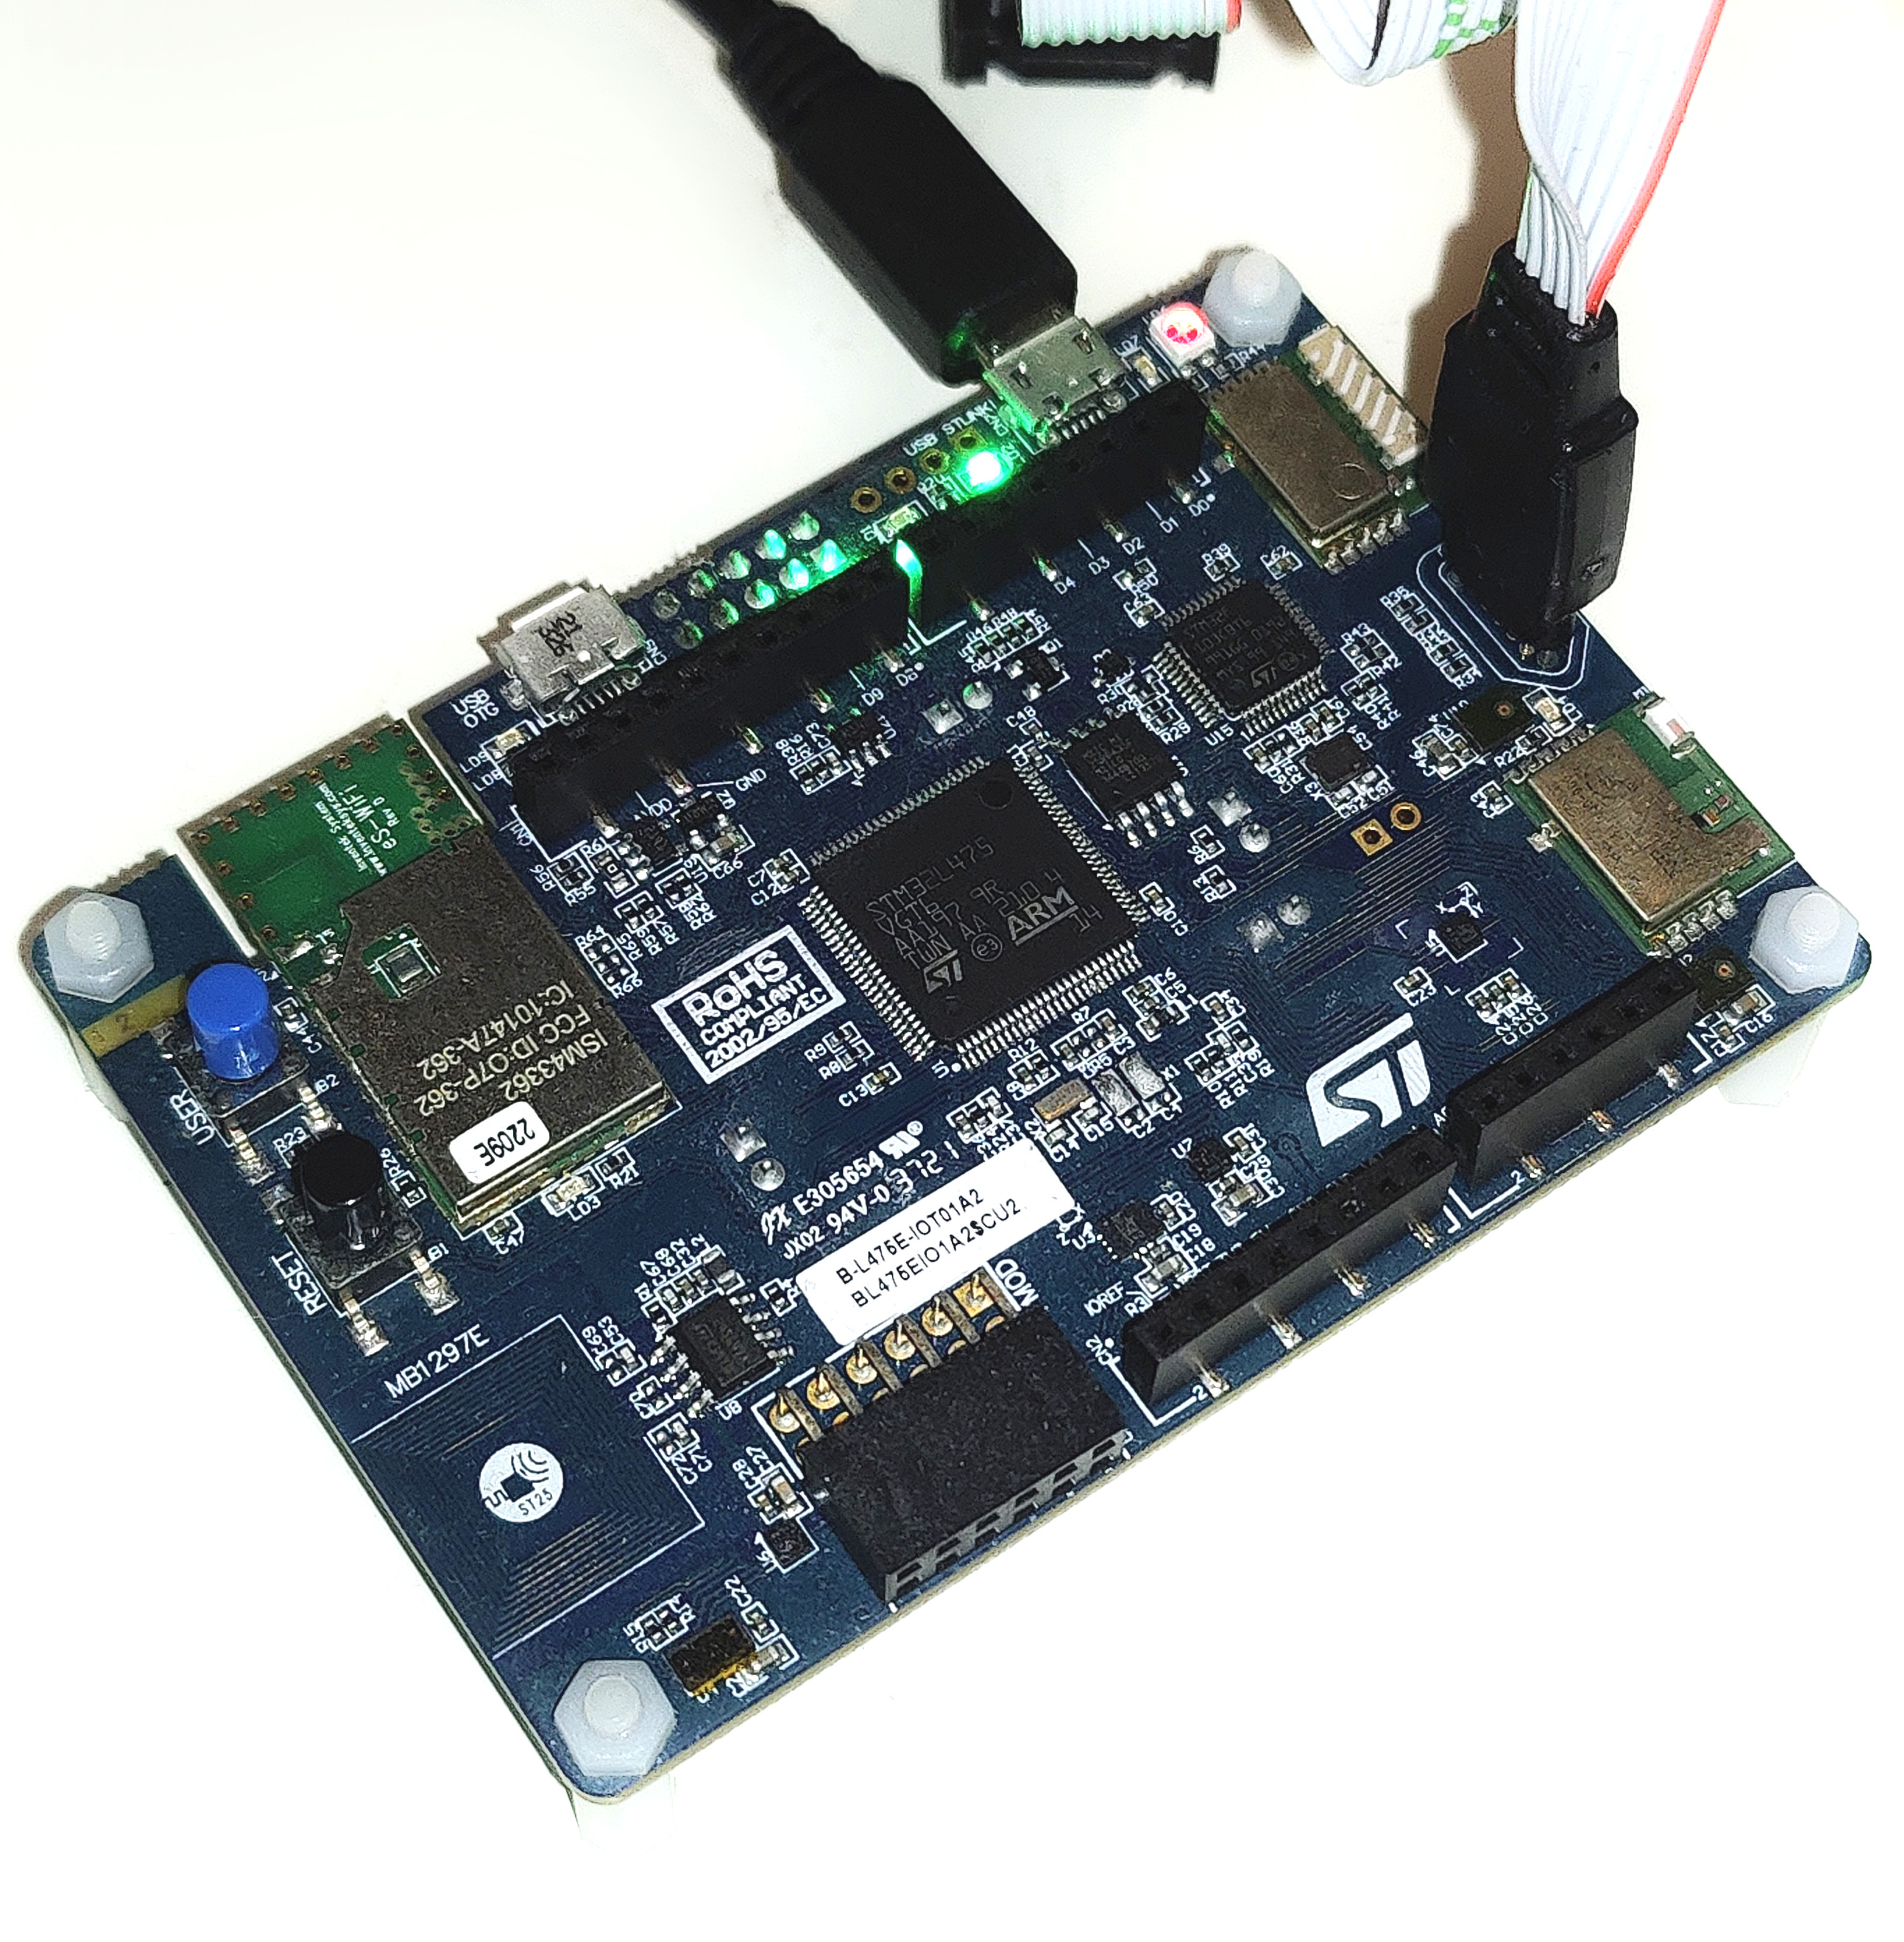
\includegraphics[width=0.9\textwidth]{figures/stm32_eval.jpg}
	\end{minipage}
\end{frame}

\section{Dataset}
\begin{frame}{Dataset}
	speech\_commands\footnote{\url{https://huggingface.co/datasets/google/speech_commands}} by P. Warden at Google.\vspace{10mm}

\begin{minipage}{0.5\textwidth}
	\setbeamercolor{local structure}{fg=mygreen}
	\setbeamercovered{transparent}

	\begin{itemize}
		\item<2-> Spoken keywords like ``yes'', ``no'', ``up'', ``down'', ...
		\item<3-> 1 second clips
		\item<4-> 16 kHz sampling rate
		\item<5-> 6:1:1 split
	\end{itemize}
	\end{minipage}
	\begin{minipage}{0.48\textwidth}
		
\includegraphics[width=0.9\textwidth]{figures/wave.png}
	\end{minipage}

\end{frame}

\section{Model and Framework}
\subsection{Framework}
\begin{frame}{Framework}

TensorFlow Lite for Microcontrollers
\begin{minipage}{0.5\textwidth}
	\setbeamercolor{local structure}{fg=mygreen}
	\setbeamercovered{transparent}
	\begin{itemize}
		\item<2->Easy to use
		\item<3->Fully customizable
		\item<4->Platform-independent
	\end{itemize}
	\end{minipage}
	\begin{minipage}{0.48\textwidth}
		
\includegraphics[width=0.9\textwidth]{figures/tensorflow.png}
	\end{minipage}

\end{frame}

\subsection{Preprocessing}
\begin{frame}{Preprocessing}
	Short-time fourier transform:\\[2mm]

$\mathbf{STFT}\{x[n]\}(m,\omega)\equiv X(m,\omega) =
\sum_{n=-\infty}^{\infty} x[n]w[n-m]e^{-i \omega n}$
	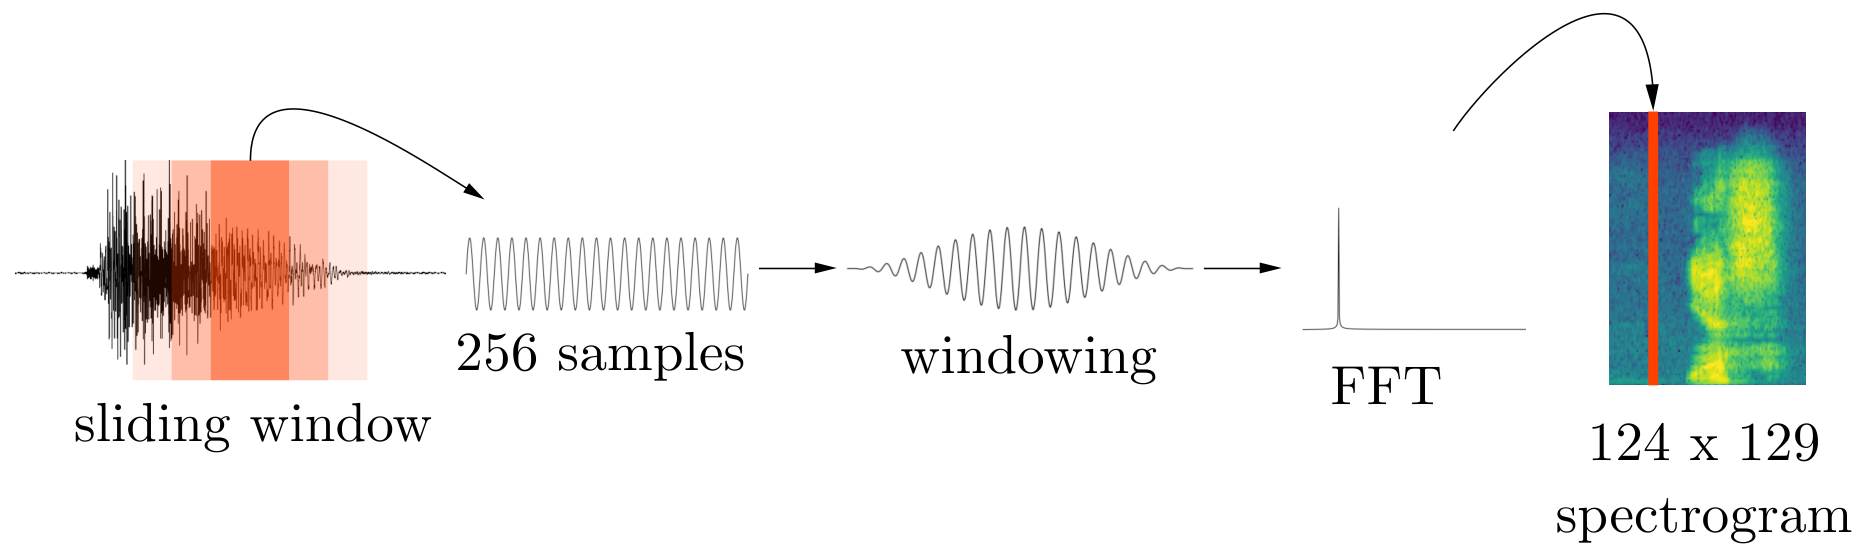
\includegraphics[width=\textwidth]{figures/stft.png}
\end{frame}

\subsection{Model}
\begin{frame}{Model}
	\begin{tikzpicture}
		\node[inner sep=0pt] at (0,0)(input){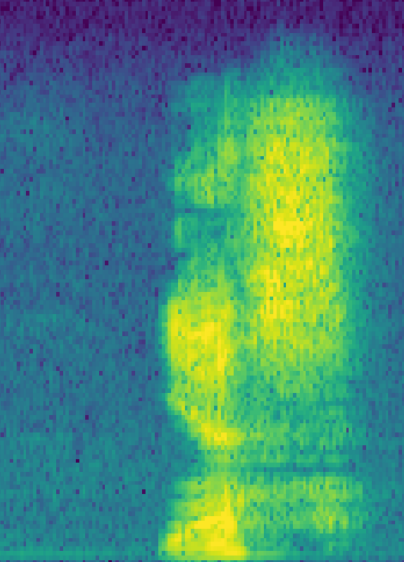
\includegraphics[width=10mm]
			{figures/spectrogram.png}};
		\node[] at (0,-1){124 x 129};
		\node[draw, thick, minimum height=10mm,visible on=<2->]
			at (1.5,0)(convA){Conv2D};
		\draw[visible on=<2->] (input.north east)--(convA.north west);
		\draw[visible on=<2->] (input.south east)--(convA.south west);

		\node[draw, thick, minimum height=5mm,visible on=<3->]
			at (3.5,0)(convB){Conv2D};
		\draw[visible on=<3->] (convA.north east)--(convB.north west);
		\draw[visible on=<3->] (convA.south east)--(convB.south west);

		\node[draw, thick, inner sep=1mm, align=center,visible on=<4->]
			at (5.5,0)(maxpool)
			{MaxPool};
		\draw[visible on=<4->] (convB.north east)--(maxpool.north west);
		\draw[visible on=<4->] (convB.south east)--(maxpool.south west);

		\node[draw, thick, minimum height=15mm, align=center,visible on=<5->]
			at (7.5,0)(dense)
			{Dense};
		\draw[visible on=<5->] (maxpool.north east)--(dense.north west);
		\draw[visible on=<5->] (maxpool.south east)--(dense.south west);

		\node[draw, thick,anchor=west,visible on=<6->] at (8.5, 2.5)(yes){YES};
		\draw[visible on=<6->] (dense.east)--(yes.west);
		\node[draw, thick,anchor=west,visible on=<6->] at (8.5, 1.5)(yes){NO};
		\draw[visible on=<6->] (dense.east)--(yes.west);
		\node[draw, thick,anchor=west,visible on=<6->] at (8.5, 0.5)(yes){UP};
		\draw[visible on=<6->] (dense.east)--(yes.west);
		\node[draw, thick,anchor=west,visible on=<6->] at (8.5, -0.5)(yes){DOWN};
		\draw[visible on=<6->] (dense.east)--(yes.west);
		\node[draw, thick,anchor=west,visible on=<6->] at (8.5, -1.5)(yes){LEFT};
		\draw[visible on=<6->] (dense.east)--(yes.west);
		\node[draw, thick,anchor=west,visible on=<6->] at (8.5, -2.5)(yes){RIGHT};
		\draw[visible on=<6->] (dense.east)--(yes.west);

	\end{tikzpicture}
\end{frame}

\section{Microcontroller Implementation}
\begin{frame}{Microcontroller Implementation}
	\setbeamercolor{local structure}{fg=mygreen}
	\setbeamercovered{transparent}
	\begin{itemize}
		\item<2->Full integer quantization of the model
		\item<3->Implemented UART protocol with CRC32 checksum
		\item<4->Preprocessing using CMSIS-DSP
	\end{itemize}
	\vspace{10mm}

	\begin{tikzpicture}
		\node[visible on=<5->] at (0,0) {
			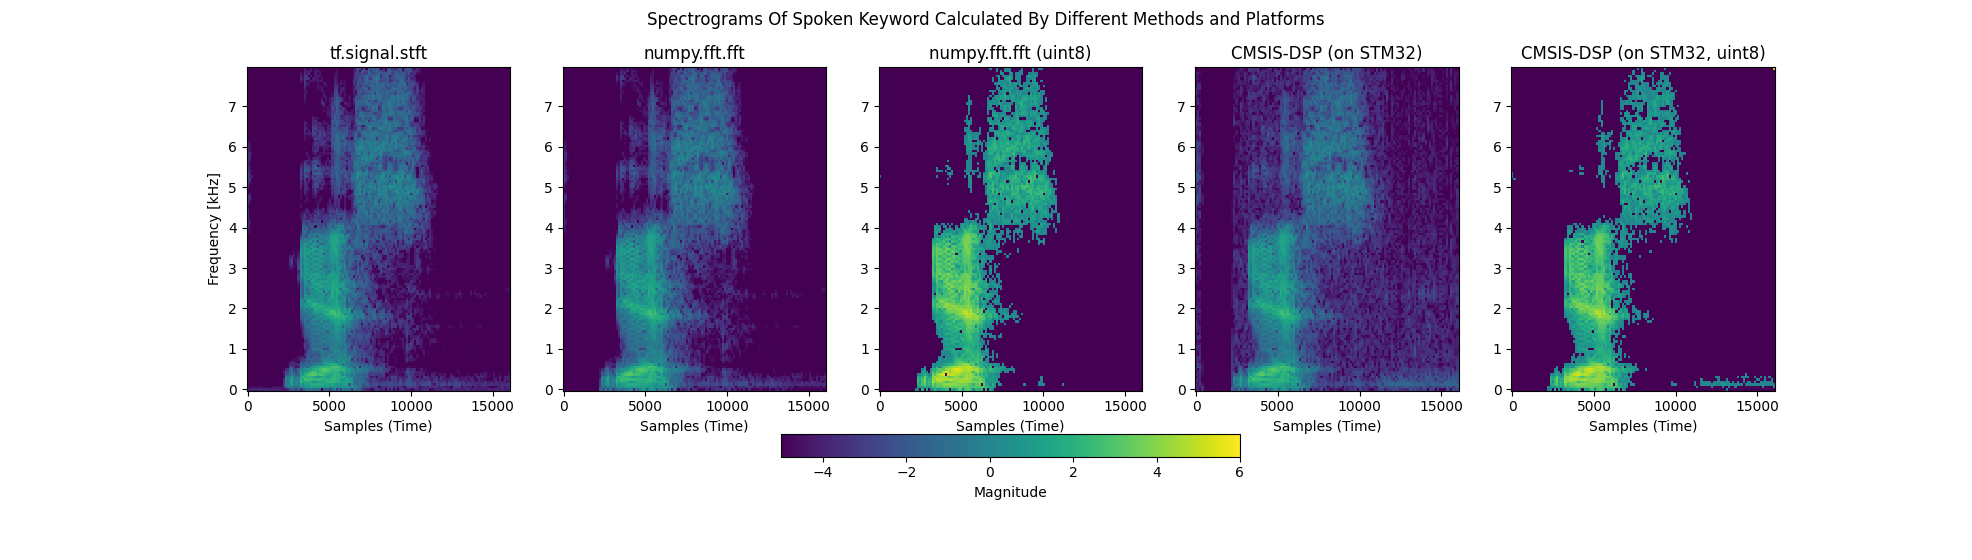
\includegraphics[width=\textwidth]{figures/spectrograms.png}};
	\end{tikzpicture}
\end{frame}

\section{Performance Evaluation}
\begin{frame}{Performance Evaluation}
	\begin{minipage}{0.32\textwidth}
	\setbeamercolor{local structure}{fg=mygreen}
	\setbeamercovered{transparent}
	\begin{itemize}
		\item<2->80.27 \% overall accuracy
		\item<3->180 ms per inference
	\end{itemize}

	\end{minipage}
	\begin{minipage}{0.65\textwidth}
		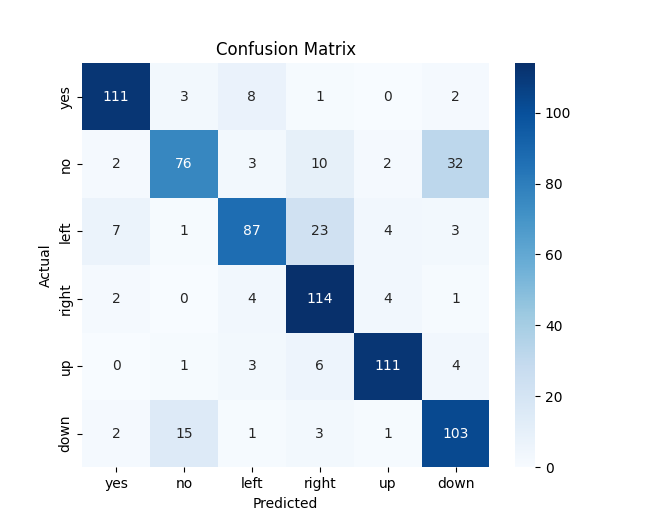
\includegraphics[width=\textwidth]{figures/confusion.png}
	\end{minipage}
\end{frame}

\begin{frame}{Memory and Storage Footprint}
	\setbeamercolor{local structure}{fg=mygreen}
	\setbeamercovered{transparent}
	\begin{itemize}
		\item<2->Limiting factor is RAM for tensor arena
		\item<3->74.5 \% SRAM used
		\item<4->45.9 \% Flash used
	\end{itemize}
	\vspace{10mm}

	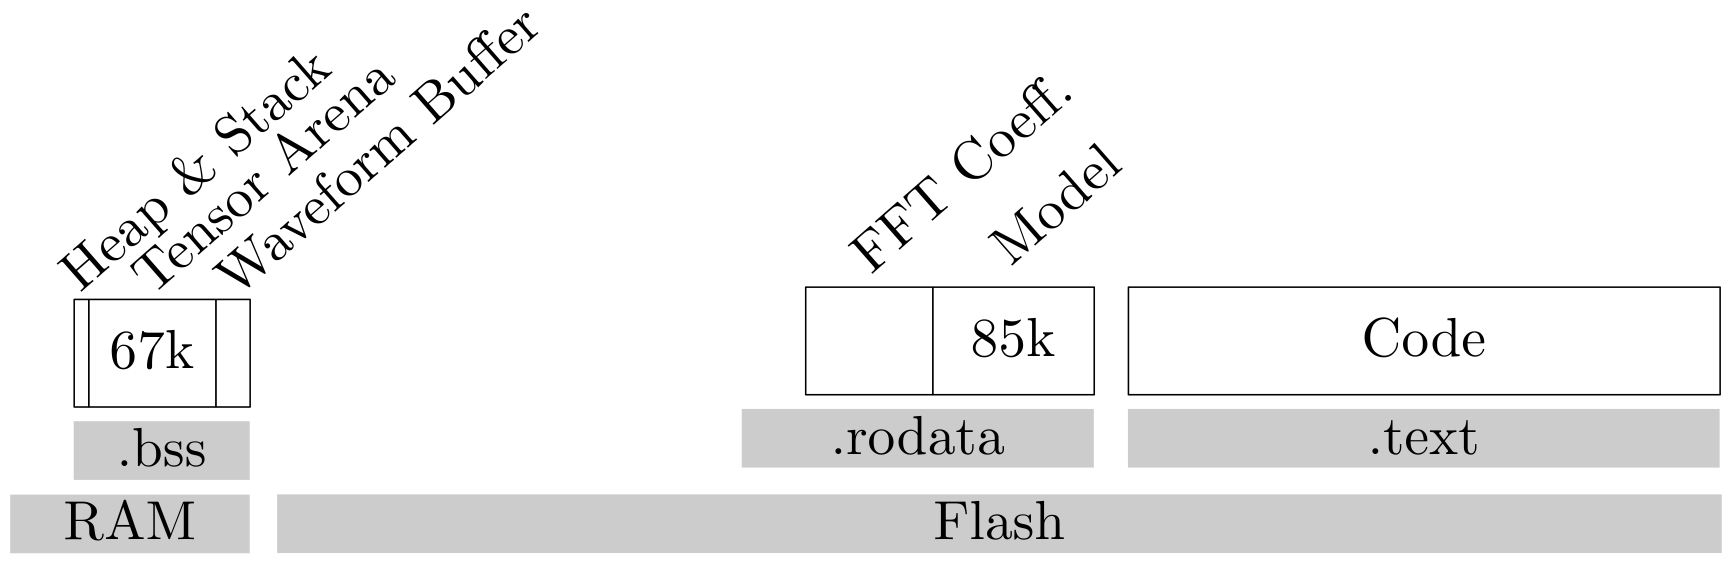
\includegraphics[width=\textwidth]{figures/memory_usage.png}
\end{frame}

\begin{frame}{Optimized TFLite Kernel (using CMSIS-NN)}
	\begin{minipage}{0.49\textwidth}
	\setbeamercolor{local structure}{fg=mygreen}
	\setbeamercovered{transparent}
	\begin{itemize}
		\item<2->Inference latency decreases by a factor of 30
		\item<3->Program size increases by 37 kiB
	\end{itemize}
	\end{minipage}
	\begin{minipage}{0.49\textwidth}
	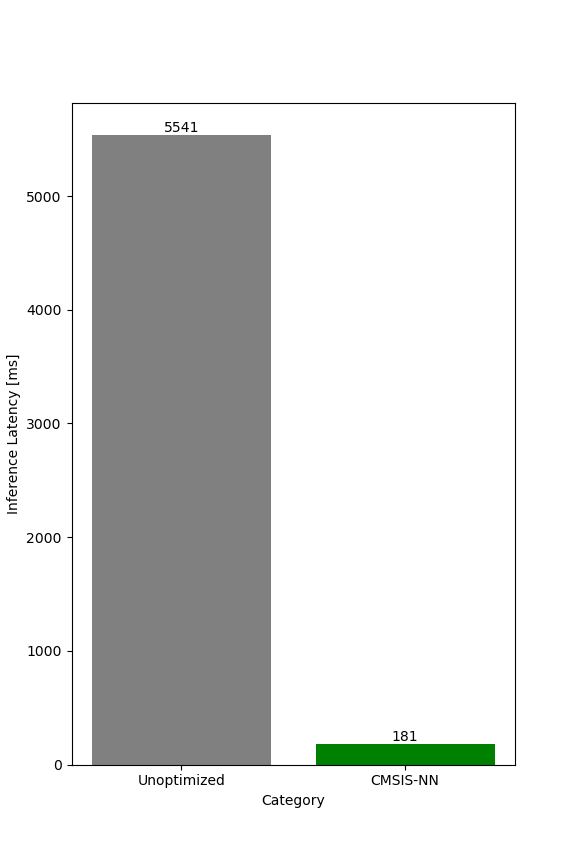
\includegraphics[width=\textwidth]{figures/optimization.png}
	\end{minipage}
\end{frame}

\section{Limitations}
\begin{frame}{Limitations}
	\setbeamercolor{local structure}{fg=mygreen}
	\setbeamercovered{transparent}
	\begin{itemize}
		\item<2->Accuracy could be better
		\item<3->``Spotting'' of keywords in background noise
		\item<4->Microphone acquisition not working
		\setbeamercolor{local structure}{fg=mygreen}
		\setbeamercovered{transparent}
		\begin{itemize}
			\item<5->Started to read out on-board PDM microphone
			\item<6->No support for 8-bit output with DMA
			\item<7->Amplitude and sampling rate seem off
		\end{itemize}

		\item<8->Optimize code, refactoring
	\end{itemize}
\end{frame}

\section{Demo}
\begin{frame}{Demo Project}
\begin{minipage}{0.49\textwidth}
	\setbeamercolor{local structure}{fg=mygreen}
	\setbeamercovered{transparent}
	\begin{itemize}
		\item<2->Not dependent on CubeIDE
		\item<3->Easy to reproduce, CMake-based build
		\item<4->CI Pipeline
		\item<5->Dependencies cleanly separated in Git submodules
	\end{itemize}
	\end{minipage}
	\begin{minipage}{0.49\textwidth}
		\centering
	
\includegraphics[width=\textwidth]{figures/github.png}
	
\includegraphics[width=0.5\textwidth]{figures/qrcode.png}
	\end{minipage}

\end{frame}

\begin{frame}{Demo}
	\begin{tikzpicture}[thick]
		\node[fill=black!10, rounded corners,
			minimum height=80mm, minimum width=40mm] at (0,0){};
		\node[fill=mygreen!25, rounded corners,
			minimum height=80mm, minimum width=40mm] at (7,0){};

		\node[anchor=north] at (7, 4){\textbf{STM32}};
		\node[anchor=north] at (0, 4){\textbf{Computer}};

		\node[] at (0,3) (mic)
			{
\includegraphics[width=5mm]{figures/microphone.png}};
		\node[] at (0,1) (wave)
			{
\includegraphics[width=30mm]{figures/wave.png}};
		\node[draw, thick,inner sep=2mm] at (7,1)(prep){Preprocessing};
		\node[inner sep=0pt] at (7,-1) (spec)
			{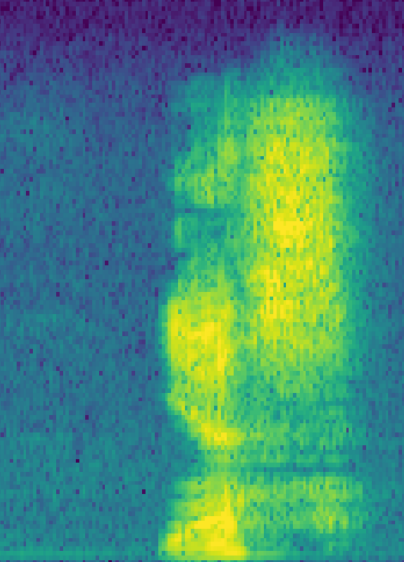
\includegraphics[width=10mm]{figures/spectrogram.png}};
		\node[draw, thick,inner sep=5mm] at (7,-3)(model){Model};

		\node[draw, thick,inner sep=5mm] at (0,-3)(result){``YES''};

		\draw[-latex](mic)--node[midway,right]{Record}(wave);
		\draw[-latex](wave)--node[midway, above]{Send waveform}(prep);
		\draw[-latex](prep)--node[midway,right]{STFT}(spec);
		\draw[-latex](spec)--node[midway,right]{}(model);
		\draw[-latex](model)--node[midway, above]{Send result}(result);

	\end{tikzpicture}
\end{frame}

\begin{frame}
	\titlepage
\end{frame}

\end{document}
